% Horizontal bar chart: success rate per metric across 9 runs
% Usage: % Horizontal bar chart: success rate per metric across 9 runs
% Usage: % Horizontal bar chart: success rate per metric across 9 runs
% Usage: % Horizontal bar chart: success rate per metric across 9 runs
% Usage: \input{generated/variability-per-metric.tex}
% Ordered by metric code (P1-P8, Q1-Q8, E1-E3)

\definecolor{cProc}{HTML}{6B9BD2}
\definecolor{cQual}{HTML}{7BC47F}
\definecolor{cConst}{HTML}{BBBBBB}

\begin{figure}[htbp]
\centering
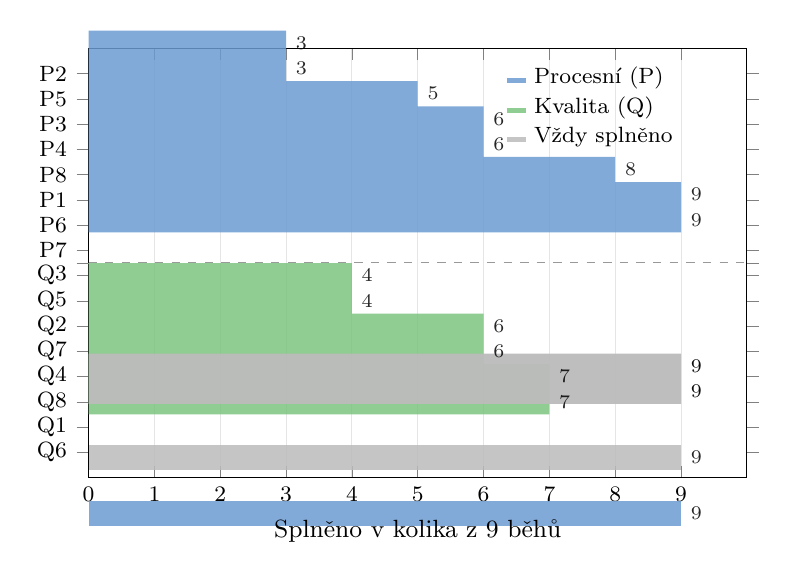
\begin{tikzpicture}
\begin{axis}[
    xbar,
    width=0.82\textwidth,
    height=0.58\textwidth,
    xlabel={Splněno v~kolika z~9 běhů},
    xmin=0, xmax=10,
    xtick={0,1,2,3,4,5,6,7,8,9},
    ytick={1,2,3,4,5,6,7,8,9,10,11,12,13,14,15,16},
    yticklabels={Q6, Q1, Q8, Q4, Q7, Q2, Q5, Q3, P7, P6, P1, P8, P4, P3, P5, P2},
    ymin=0, ymax=17,
    yticklabel style={font=\footnotesize},
    xticklabel style={font=\footnotesize},
    xlabel style={font=\small},
    bar width=9pt,
    nodes near coords,
    nodes near coords style={font=\scriptsize, anchor=west},
    xmajorgrids=true,
    ymajorgrids=false,
    grid style={gray!20},
    clip=false,
    % Horizontal separator between P and Q groups
    extra y ticks={8.5},
    extra y tick labels={},
    extra y tick style={grid=major, grid style={black!40, dashed}},
]

% P metrics (blue) — P1 through P8, bottom to top = P2,P5,P3,P4,P8,P1,P6,P7
\addplot[draw=none, fill=cProc, fill opacity=0.85] coordinates {
    (9,1)   % Q6
};
\addplot[draw=none, fill=cConst, fill opacity=0.85] coordinates {
    (9,2)   % Q1
};
\addplot[draw=none, fill=cQual, fill opacity=0.85] coordinates {
    (7,3)   % Q8
    (7,4)   % Q4
    (6,5)   % Q7
    (6,6)   % Q2
    (4,7)   % Q5
    (4,8)   % Q3
};
\addplot[draw=none, fill=cProc, fill opacity=0.85] coordinates {
    (9,9)   % P7
    (9,10)  % P6
    (8,11)  % P1
    (6,12)  % P8
    (6,13)  % P4
    (5,14)  % P3
    (3,15)  % P5
    (3,16)  % P2
};

% Fix: Q6 and Q1 should be gray (always met)
% Redraw Q6 and Q1 in gray on top
\addplot[draw=none, fill=cConst, fill opacity=0.95] coordinates {
    (9,1)   % Q6
    (9,2)   % Q1
};

% Manual legend
\node[anchor=north west, font=\footnotesize] at (rel axis cs:0.62,0.98) {
    \tikz{\fill[cProc, fill opacity=0.85] (0,0) rectangle (0.3,0.2);} Procesní (P)
};
\node[anchor=north west, font=\footnotesize] at (rel axis cs:0.62,0.91) {
    \tikz{\fill[cQual, fill opacity=0.85] (0,0) rectangle (0.3,0.2);} Kvalita (Q)
};
\node[anchor=north west, font=\footnotesize] at (rel axis cs:0.62,0.84) {
    \tikz{\fill[cConst, fill opacity=0.85] (0,0) rectangle (0.3,0.2);} Vždy splněno
};

\end{axis}
\end{tikzpicture}
\caption{Míra splnění jednotlivých metrik napříč devíti běhy.
Procesní metriky \acs{P2} a~\acs{P5} byly splněny nejméně často
(3/9), zatímco \acs{Q1} a~\acs{Q6} zůstaly stabilní ve všech
bězích. Přerušovaná čára odděluje procesní a~produktové metriky.}
\label{fig:variability-per-metric}
\end{figure}

% Ordered by metric code (P1-P8, Q1-Q8, E1-E3)

\definecolor{cProc}{HTML}{6B9BD2}
\definecolor{cQual}{HTML}{7BC47F}
\definecolor{cConst}{HTML}{BBBBBB}

\begin{figure}[htbp]
\centering
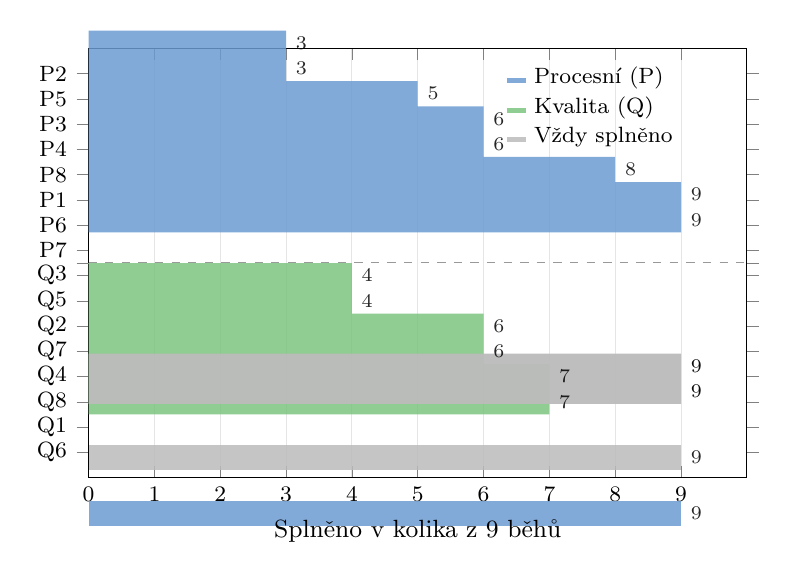
\begin{tikzpicture}
\begin{axis}[
    xbar,
    width=0.82\textwidth,
    height=0.58\textwidth,
    xlabel={Splněno v~kolika z~9 běhů},
    xmin=0, xmax=10,
    xtick={0,1,2,3,4,5,6,7,8,9},
    ytick={1,2,3,4,5,6,7,8,9,10,11,12,13,14,15,16},
    yticklabels={Q6, Q1, Q8, Q4, Q7, Q2, Q5, Q3, P7, P6, P1, P8, P4, P3, P5, P2},
    ymin=0, ymax=17,
    yticklabel style={font=\footnotesize},
    xticklabel style={font=\footnotesize},
    xlabel style={font=\small},
    bar width=9pt,
    nodes near coords,
    nodes near coords style={font=\scriptsize, anchor=west},
    xmajorgrids=true,
    ymajorgrids=false,
    grid style={gray!20},
    clip=false,
    % Horizontal separator between P and Q groups
    extra y ticks={8.5},
    extra y tick labels={},
    extra y tick style={grid=major, grid style={black!40, dashed}},
]

% P metrics (blue) — P1 through P8, bottom to top = P2,P5,P3,P4,P8,P1,P6,P7
\addplot[draw=none, fill=cProc, fill opacity=0.85] coordinates {
    (9,1)   % Q6
};
\addplot[draw=none, fill=cConst, fill opacity=0.85] coordinates {
    (9,2)   % Q1
};
\addplot[draw=none, fill=cQual, fill opacity=0.85] coordinates {
    (7,3)   % Q8
    (7,4)   % Q4
    (6,5)   % Q7
    (6,6)   % Q2
    (4,7)   % Q5
    (4,8)   % Q3
};
\addplot[draw=none, fill=cProc, fill opacity=0.85] coordinates {
    (9,9)   % P7
    (9,10)  % P6
    (8,11)  % P1
    (6,12)  % P8
    (6,13)  % P4
    (5,14)  % P3
    (3,15)  % P5
    (3,16)  % P2
};

% Fix: Q6 and Q1 should be gray (always met)
% Redraw Q6 and Q1 in gray on top
\addplot[draw=none, fill=cConst, fill opacity=0.95] coordinates {
    (9,1)   % Q6
    (9,2)   % Q1
};

% Manual legend
\node[anchor=north west, font=\footnotesize] at (rel axis cs:0.62,0.98) {
    \tikz{\fill[cProc, fill opacity=0.85] (0,0) rectangle (0.3,0.2);} Procesní (P)
};
\node[anchor=north west, font=\footnotesize] at (rel axis cs:0.62,0.91) {
    \tikz{\fill[cQual, fill opacity=0.85] (0,0) rectangle (0.3,0.2);} Kvalita (Q)
};
\node[anchor=north west, font=\footnotesize] at (rel axis cs:0.62,0.84) {
    \tikz{\fill[cConst, fill opacity=0.85] (0,0) rectangle (0.3,0.2);} Vždy splněno
};

\end{axis}
\end{tikzpicture}
\caption{Míra splnění jednotlivých metrik napříč devíti běhy.
Procesní metriky \acs{P2} a~\acs{P5} byly splněny nejméně často
(3/9), zatímco \acs{Q1} a~\acs{Q6} zůstaly stabilní ve všech
bězích. Přerušovaná čára odděluje procesní a~produktové metriky.}
\label{fig:variability-per-metric}
\end{figure}

% Ordered by metric code (P1-P8, Q1-Q8, E1-E3)

\definecolor{cProc}{HTML}{6B9BD2}
\definecolor{cQual}{HTML}{7BC47F}
\definecolor{cConst}{HTML}{BBBBBB}

\begin{figure}[htbp]
\centering
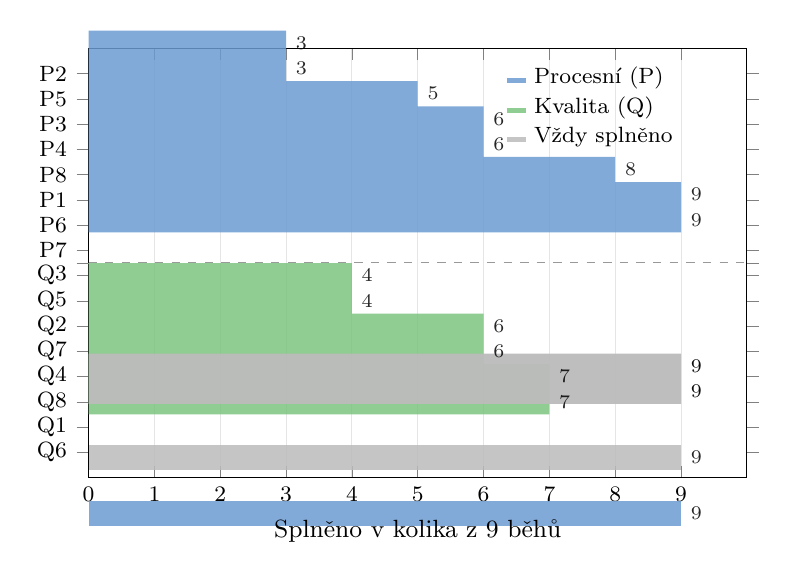
\begin{tikzpicture}
\begin{axis}[
    xbar,
    width=0.82\textwidth,
    height=0.58\textwidth,
    xlabel={Splněno v~kolika z~9 běhů},
    xmin=0, xmax=10,
    xtick={0,1,2,3,4,5,6,7,8,9},
    ytick={1,2,3,4,5,6,7,8,9,10,11,12,13,14,15,16},
    yticklabels={Q6, Q1, Q8, Q4, Q7, Q2, Q5, Q3, P7, P6, P1, P8, P4, P3, P5, P2},
    ymin=0, ymax=17,
    yticklabel style={font=\footnotesize},
    xticklabel style={font=\footnotesize},
    xlabel style={font=\small},
    bar width=9pt,
    nodes near coords,
    nodes near coords style={font=\scriptsize, anchor=west},
    xmajorgrids=true,
    ymajorgrids=false,
    grid style={gray!20},
    clip=false,
    % Horizontal separator between P and Q groups
    extra y ticks={8.5},
    extra y tick labels={},
    extra y tick style={grid=major, grid style={black!40, dashed}},
]

% P metrics (blue) — P1 through P8, bottom to top = P2,P5,P3,P4,P8,P1,P6,P7
\addplot[draw=none, fill=cProc, fill opacity=0.85] coordinates {
    (9,1)   % Q6
};
\addplot[draw=none, fill=cConst, fill opacity=0.85] coordinates {
    (9,2)   % Q1
};
\addplot[draw=none, fill=cQual, fill opacity=0.85] coordinates {
    (7,3)   % Q8
    (7,4)   % Q4
    (6,5)   % Q7
    (6,6)   % Q2
    (4,7)   % Q5
    (4,8)   % Q3
};
\addplot[draw=none, fill=cProc, fill opacity=0.85] coordinates {
    (9,9)   % P7
    (9,10)  % P6
    (8,11)  % P1
    (6,12)  % P8
    (6,13)  % P4
    (5,14)  % P3
    (3,15)  % P5
    (3,16)  % P2
};

% Fix: Q6 and Q1 should be gray (always met)
% Redraw Q6 and Q1 in gray on top
\addplot[draw=none, fill=cConst, fill opacity=0.95] coordinates {
    (9,1)   % Q6
    (9,2)   % Q1
};

% Manual legend
\node[anchor=north west, font=\footnotesize] at (rel axis cs:0.62,0.98) {
    \tikz{\fill[cProc, fill opacity=0.85] (0,0) rectangle (0.3,0.2);} Procesní (P)
};
\node[anchor=north west, font=\footnotesize] at (rel axis cs:0.62,0.91) {
    \tikz{\fill[cQual, fill opacity=0.85] (0,0) rectangle (0.3,0.2);} Kvalita (Q)
};
\node[anchor=north west, font=\footnotesize] at (rel axis cs:0.62,0.84) {
    \tikz{\fill[cConst, fill opacity=0.85] (0,0) rectangle (0.3,0.2);} Vždy splněno
};

\end{axis}
\end{tikzpicture}
\caption{Míra splnění jednotlivých metrik napříč devíti běhy.
Procesní metriky \acs{P2} a~\acs{P5} byly splněny nejméně často
(3/9), zatímco \acs{Q1} a~\acs{Q6} zůstaly stabilní ve všech
bězích. Přerušovaná čára odděluje procesní a~produktové metriky.}
\label{fig:variability-per-metric}
\end{figure}

% Ordered by metric code (P1-P8, Q1-Q8, E1-E3)

\definecolor{cProc}{HTML}{6B9BD2}
\definecolor{cQual}{HTML}{7BC47F}
\definecolor{cConst}{HTML}{BBBBBB}

\begin{figure}[htbp]
\centering
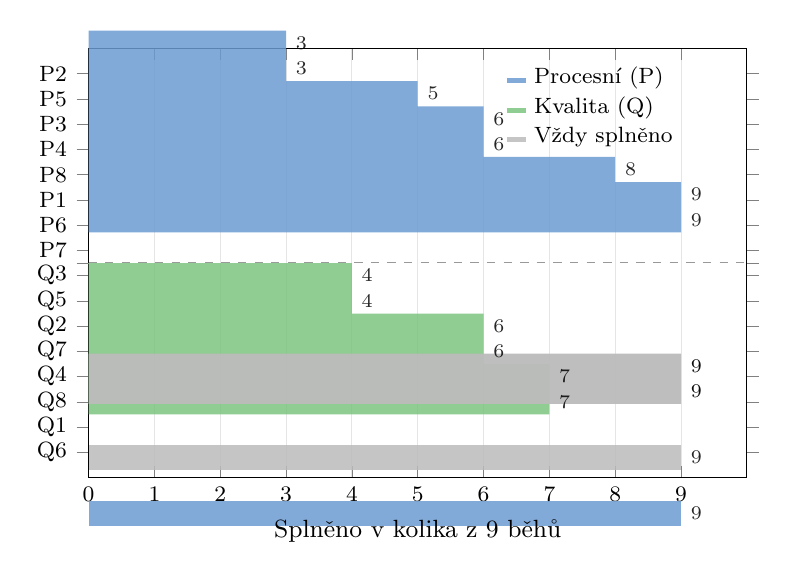
\begin{tikzpicture}
\begin{axis}[
    xbar,
    width=0.82\textwidth,
    height=0.58\textwidth,
    xlabel={Splněno v~kolika z~9 běhů},
    xmin=0, xmax=10,
    xtick={0,1,2,3,4,5,6,7,8,9},
    ytick={1,2,3,4,5,6,7,8,9,10,11,12,13,14,15,16},
    yticklabels={Q6, Q1, Q8, Q4, Q7, Q2, Q5, Q3, P7, P6, P1, P8, P4, P3, P5, P2},
    ymin=0, ymax=17,
    yticklabel style={font=\footnotesize},
    xticklabel style={font=\footnotesize},
    xlabel style={font=\small},
    bar width=9pt,
    nodes near coords,
    nodes near coords style={font=\scriptsize, anchor=west},
    xmajorgrids=true,
    ymajorgrids=false,
    grid style={gray!20},
    clip=false,
    % Horizontal separator between P and Q groups
    extra y ticks={8.5},
    extra y tick labels={},
    extra y tick style={grid=major, grid style={black!40, dashed}},
]

% P metrics (blue) — P1 through P8, bottom to top = P2,P5,P3,P4,P8,P1,P6,P7
\addplot[draw=none, fill=cProc, fill opacity=0.85] coordinates {
    (9,1)   % Q6
};
\addplot[draw=none, fill=cConst, fill opacity=0.85] coordinates {
    (9,2)   % Q1
};
\addplot[draw=none, fill=cQual, fill opacity=0.85] coordinates {
    (7,3)   % Q8
    (7,4)   % Q4
    (6,5)   % Q7
    (6,6)   % Q2
    (4,7)   % Q5
    (4,8)   % Q3
};
\addplot[draw=none, fill=cProc, fill opacity=0.85] coordinates {
    (9,9)   % P7
    (9,10)  % P6
    (8,11)  % P1
    (6,12)  % P8
    (6,13)  % P4
    (5,14)  % P3
    (3,15)  % P5
    (3,16)  % P2
};

% Fix: Q6 and Q1 should be gray (always met)
% Redraw Q6 and Q1 in gray on top
\addplot[draw=none, fill=cConst, fill opacity=0.95] coordinates {
    (9,1)   % Q6
    (9,2)   % Q1
};

% Manual legend
\node[anchor=north west, font=\footnotesize] at (rel axis cs:0.62,0.98) {
    \tikz{\fill[cProc, fill opacity=0.85] (0,0) rectangle (0.3,0.2);} Procesní (P)
};
\node[anchor=north west, font=\footnotesize] at (rel axis cs:0.62,0.91) {
    \tikz{\fill[cQual, fill opacity=0.85] (0,0) rectangle (0.3,0.2);} Kvalita (Q)
};
\node[anchor=north west, font=\footnotesize] at (rel axis cs:0.62,0.84) {
    \tikz{\fill[cConst, fill opacity=0.85] (0,0) rectangle (0.3,0.2);} Vždy splněno
};

\end{axis}
\end{tikzpicture}
\caption{Míra splnění jednotlivých metrik napříč devíti běhy.
Procesní metriky \acs{P2} a~\acs{P5} byly splněny nejméně často
(3/9), zatímco \acs{Q1} a~\acs{Q6} zůstaly stabilní ve všech
bězích. Přerušovaná čára odděluje procesní a~produktové metriky.}
\label{fig:variability-per-metric}
\end{figure}
